\documentclass[english,notitlepage,aps,pra,10pt]{revtex4-2}
%For preview: skriv i terminal: latexmk -pdf -pvc filnavn

% if you want a single-column, remove reprint

% allows special characters (including æøå)
%\usepackage[utf8]{inputenc}
%\usepackage[english]{babel}

%% note that you may need to download some of these packages manually, it depends on your setup.
%% I recommend downloading TeXMaker, because it includes a large library of the most common packages.

\usepackage{physics,amssymb}  % mathematical symbols (physics imports amsmath)
\usepackage{amsmath}
% \usepackage{amssymb}
\usepackage{graphicx}         % include graphics such as plots
\usepackage{xcolor}           % set colors
\usepackage{hyperref}         % automagic cross-referencing (this is GODLIKE)
\usepackage{listings}         % display code
\usepackage{subfigure}        % imports a lot of cool and useful figure commands
\usepackage{float}
%\usepackage[section]{placeins}
\usepackage{algorithm}
\usepackage[noend]{algpseudocode}
\usepackage{subfigure}
\usepackage{tikz}
\usetikzlibrary{quantikz}
% defines the color of hyperref objects
% Blending two colors:  blue!80!black  =  80% blue and 20% black
\hypersetup{ % this is just my personal choice, feel free to change things
    colorlinks,
    linkcolor={red!50!black},
    citecolor={blue!50!black},
    urlcolor={blue!80!black}}

%% Defines the style of the programming listing
%% This is actually my personal template, go ahead and change stuff if you want



%% USEFUL LINKS:
%%
%%   UiO LaTeX guides:        https://www.mn.uio.no/ifi/tjenester/it/hjelp/latex/
%%   mathematics:             https://en.wikibooks.org/wiki/LaTeX/Mathematics

%%   PHYSICS !                https://mirror.hmc.edu/ctan/macros/latex/contrib/physics/physics.pdf

%%   the basics of Tikz:       https://en.wikibooks.org/wiki/LaTeX/PGF/Tikz
%%   all the colors!:          https://en.wikibooks.org/wiki/LaTeX/Colors
%%   how to draw tables:       https://en.wikibooks.org/wiki/LaTeX/Tables
%%   code listing styles:      https://en.wikibooks.org/wiki/LaTeX/Source_Code_Listings
%%   \includegraphics          https://en.wikibooks.org/wiki/LaTeX/Importing_Graphics
%%   learn more about figures  https://en.wikibooks.org/wiki/LaTeX/Floats,_Figures_and_Captions
%%   automagic bibliography:   https://en.wikibooks.org/wiki/LaTeX/Bibliography_Management  (this one is kinda difficult the first time)
%%   REVTeX Guide:             http://www.physics.csbsju.edu/370/papers/Journal_Style_Manuals/auguide4-1.pdf
%%
%%   (this document is of class "revtex4-1", the REVTeX Guide explains how the class works)


%% CREATING THE .pdf FILE USING LINUX IN THE TERMINAL
%%
%% [terminal]$ pdflatex template.tex
%%
%% Run the command twice, always.
%% If you want to use \footnote, you need to run these commands (IN THIS SPECIFIC ORDER)
%%
%% [terminal]$ pdflatex template.tex
%% [terminal]$ bibtex template
%% [terminal]$ pdflatex template.tex
%% [terminal]$ pdflatex template.tex
%%
%% Don't ask me why, I don't know.

\newcommand{\e}{\mathrm{e}}
\newcommand{\bv}[1]{\mathbf{#1}}


\begin{document}

\title{FYS4150 - Project 1}      % self-explanatory
\author{Halvor Melkild}          % self-explanatory
\date{\today}                             % self-explanatory
\noaffiliation                            % ignore this, but keep it.


\maketitle

\textit{GitHub repo: \href{https://github.com/halvorme/FYS4150/}{https://github.com/halvorme/FYS4150}}

\section*{Problem 1}

We are looking at the one-dimensional Poisson equation 
\begin{equation}
    -\dv[2]{u}{x} = f(x),
    \label{eq:poisson}
\end{equation}
on the range $x \in [0,1]$. The boudary conditions are $u(0) = u(1) = 0$ and source term is chosen as 
\begin{equation}
    f(x) = 100\, \e^{-10x}.
\end{equation}
An exact solution to Equation~\ref{eq:poisson} has the form 
\begin{equation}
    u(x) = -\e^{-10x} + C_1 x + C_2.
\end{equation}
The boundary condition at $x=0$ gives that $C_2 = 1$, and the condition at $x=1$ then gives that $C_1 = \e^{-10} - 1$. It follows that 
\begin{equation}
    u(x) = 1 - (1-\e^{-10})x - \e^{-10x} 
\end{equation}
is a solution to Equation~\ref{eq:poisson}, satisfying the given boundary conditions.


\section*{Problem 2}

The plot of the exact solution is seen in Figure~\ref{fig:uExact}. The generating code is found in the repository linked at the top of the document.

\begin{figure}%[h!]
    \begin{center}
        \includegraphics{../imgs/u_exact.pdf}
        \caption{The plot shows the exact solution to the Poisson equation (Eq.~\ref{eq:poisson}), with the source term $f(x) = 100 \e^{-10x}$, and boundary conditions $u(0)=u(1)=0$.}
        \label{fig:uExact}     
    \end{center}
\end{figure}


\section*{Problem 3}

To make a discretised version of the Poisson equation, we need to discretise the second derivative. We start out with the definition of the derivative
\begin{equation}
    u'(x) = \dv{u}{x} = \lim_{\Delta x \to 0} \frac{u(x+\Delta x) - u(x)}{\Delta x}.
\end{equation}
If a function is differentiable at a point $x$ it means that the limit has to be the same if you approach $x$ from above or below. It follows that 
\begin{equation}
    u'(x) = \lim_{\Delta x \to 0} \frac{u(x) - u(x-\Delta x)}{\Delta x}
\end{equation}
is an equivalent definition. The second derivative can then be defined the following way,
\begin{equation}
    \begin{split}
        u''(x) = \dv[2]{u}{x} &= \lim_{\Delta x \to 0} \frac{u'(x+\Delta x) - u'(x)}{\Delta x} \\
            &= \lim_{\Delta x \to 0} \frac{u(x+\Delta x) - 2u(x) + u(x-\Delta x)}{\Delta x^2}.
    \end{split}
    \label{eq:secDer}
\end{equation}
When we discretise the $x$-axis it will no longer be possible to take the limit $\Delta x \to 0$. The smallest possible value is $\Delta x = h$, where $h$ is the stepsize of the discretisation. We will than have to find an approximation for $u''(x)$. By Taylor expanding 

We would now like to discretise this expression. We start by discretising the $x$-axis. The line segment $[1,0]$ is replaced by the set with $N+1$ elements, 
\begin{equation}
    \{x_i = i h \mid i\in\{0,1, \dots, N\},\ h = \frac{1}{N}\}.
\end{equation}
The distance between each point is given by $h$. We notice that $x_i + nh = x_{i+n}$ for any integer $n$. The function $u(x)$ is now replaced by the set
\begin{equation}
    v_i = u(x_i),
\end{equation}
where we choose denote the solution to the discretised equation as $v$. The boundary conditions tells us that $v_0 = v_N = 0$. For the source term we will simply use $f_i = f(x_i)$. 

When the function $u(x)$ is discretised, we can't take the limit $\Delta x \to 0$ any more. The best we can do is $\Delta x \to h$. We than has to work with an approximation to Equation~\ref{eq:secDer}. By Taylor expanding 
\begin{equation}
    u(x \pm h) = u(x) \pm h u'(x) + \frac{1}{2} h^2 u''(x) \pm \frac{1}{6} h^3 u^{(3)}(x) + \frac{1}{24} h^4 u^{(4)} + \mathcal{O}(h^5)
\end{equation}
we find that 
\begin{equation}
    u''(x) = \frac{u(x+h) - 2u(x) + u(x-h)}{h^2} + \mathcal{O}(h^2).
    \label{eq:approxDeriv}
\end{equation}
Discarding the terms of $\mathcal{O}(h^2)$ and discretising the remainding expression we get
\begin{equation}
    v_i'' = \frac{1}{h^2}(v_{i+1} - 2v_i + v_{i-1}).
\end{equation}

In the end, the discretised Poisson equation (Eq.~\ref{eq:poisson}) can be written as
\begin{equation}
    -v_{i-1} + 2v_i - v_{i+1} = h^2 f_i,
    \label{eq:discPoisson}
\end{equation} 
where $i \in \{1,\dots, N-1\}$.


\section*{Problem 4}

The discretised Poisson equation (Eq.~\ref{eq:discPoisson}) gives us a set of $N-1$ equations, with $N-1$ unknowns, as $v_0$ and $v_N$ are set by the boundary conditions. We can write each of these equation on matrix form
\begin{equation}
    \begin{pmatrix}
        -1 & 2 & -1
    \end{pmatrix}
    \begin{pmatrix}
        v_{i-1} \\
        v_i \\
        v_{i+1}
    \end{pmatrix}
    = h^2 f_i.
\end{equation} 
For the first and last equation we can use the boundary conditions and simplify them as  
\begin{equation}
    \begin{split}
        \begin{pmatrix}
            2 & -1
        \end{pmatrix}
        \begin{pmatrix}
            v_1 \\
            v_2
        \end{pmatrix}
        &= h^2 f_1, \\
        \begin{pmatrix}
            -1 & 2
        \end{pmatrix}
        \begin{pmatrix}
            v_{N-2} \\
            v_{N-1}
        \end{pmatrix}
        &= h^2 f_{N-1}.
    \end{split}
\end{equation}
Stacking all these equations in one matrix we get 
\begin{equation}
    \begin{pmatrix}
         2 & -1 &  0 &  0 & \cdots &  0 &  0 \\
        -1 &  2 & -1 &  0 & \cdots &  0 &  0 \\
         0 & -1 &  2 & -1 & \cdots &  0 &  0 \\
         0 &  0 & -1 &  2 & \cdots &  0 &  0 \\
        \vdots & \vdots & \vdots & \vdots & \ddots & \vdots  & \vdots\\
         0 &  0 &  0 &  0 & \cdots &  2 & -1 \\
         0 &  0 &  0 &  0 & \cdots & -1 &  2 \\
    \end{pmatrix}
    \begin{pmatrix}
        v_1 \\
        v_2 \\
        v_3 \\
        v_4 \\
        \vdots \\
        v_{N-2} \\
        v_{N-1}
    \end{pmatrix}
    =
    h^2
    \begin{pmatrix}
        f_1 \\
        f_2 \\
        f_3 \\
        f_4 \\
        \vdots \\
        f_{N-2} \\
        f_{N-1}
    \end{pmatrix}.
    \label{eq:discPoissonMat}
\end{equation}
By discretising the Poisson equation we could rewrite it as matrix equation with the form 
\begin{equation}
    A \bv{v} = \bv{g},
\end{equation}
where $A$ is a tridiagonal matrix, $\bv{v}$ is a vector of the unknown $v_i$'s and $\bv{g}$ encodes the information of the source term, but is scaled by a factor $h^2$. 


\section*{Problem 5}

The vector $\bv{v}$, as defined above, includes only the subset of internal points of $v$, which are unknown. The complete solution $\bv{v}^*$, with length $m$, also includes the two endpoints, $v_0$ and $v_N$, which are determined by the boundary conditions. That means
\begin{equation}
    m = n + 2 = N + 1.
\end{equation}


\section*{Problem 6}
\subsection*{Problem a}
We want an algorithm to solve the general matrix equation 
\begin{equation}
    A \bv{v} = \bv{g},
    \label{eq:AvEqg}
\end{equation}
where $A$ is a $n \times n$ tridiagonal matrix. We denote the subdiagonal, main diagonal and superdiagonal as $\bv{a}$, $\bv{b}$ and $\bv{c}$, respectively. The vectors $\bv{v}$, $\bv{g}$ and $\bv{b}$ has length $n$, and the off-diagonal vectors $\bv{a}$ and $\bv{c}$ has length $n-1$. 

To solve Equation~\ref{eq:AvEqg} we simply us Gaussian elimination. The algorithm is separated in forward and backward substitution. In the forward substitution, the subdiagonal $\bv{a}$ is eliminated, while $\bv{b}$ and $\bv{g}$ are modified. In the backward substitution, we solve each row for $v_i$, one after the other. The exact steps are presented in Algorithm~\ref{algo:triDiagGauss}.

\begin{algorithm}[H]
    \caption{Gaussian elimination of a tridiagonal matrix}\label{algo:triDiagGauss}
    \begin{algorithmic}
        \State Initialise $\bv{a}$, $\bv{b}$, $\bv{c}$ and $\bv{g}$ with their given values
        \State Initialise new vector $\bv{v}$ of length $n$ 

        \Comment Forward substitution
        \For{$i = 1, 2, \dots, n-1$}                    \Comment $n-1$ iterations
            \State $d = a_i/b_i$                        \Comment 1 FLOP
            \State $b_{i+1} = b_{i+1} - d\, c_i$        \Comment 2 FLOPs 
            \State $g_{i+1} = g_{i+1} - d\, g_i$        \Comment 2 FLOPs 
        \EndFor
        \Comment Backward substitution
        \State $v_n = g_n/b_n$                          \Comment 1 FLOP 
        \For{$i = 1, 2, \dots, n-1$}                    \Comment $n-1$ iterations
            \State $v_{n-i} = (g_{n-i} - c_{n-i} v_{n-i+1})/b_{n-i}$  \Comment 3 FLOPs
        \EndFor
    \end{algorithmic}
\end{algorithm}

\subsection*{Problem b}

In the right coloumn of Algorithm~\ref{algo:triDiagGauss} we have listed the number of floating-point operations (FLOPs) needed for each step. We see that there are $5(n-1)$ FLOPs needed for the forward substitution and $3(n-1)+1$ for backwards substitution. When we sum these, we find that the algorithm needs
\begin{equation}
    (8n-7) \textrm{ FLOPs}.
    \label{eq:genFlop}
\end{equation} 
We note that the number of FLOPs depends linearly on $n$.


\section*{Problem 7}

The alogrithm is implemented in the function \verb+genAlgo+, found in the file \verb+algo.cpp+ in the repo. The resulting plot is found in Figure~\ref{fig:v}.

\begin{figure}%[h!]
    \begin{center}
        \includegraphics{../imgs/v.pdf}
        \caption{The plot shows the exact solution $u(x)$ to the Poisson equation and the numerical approximation $v(x)$ for three different stepsizes.}
        \label{fig:v}
    \end{center}
\end{figure}


\section*{Problem 8}

The plots of the absolute error 
\begin{equation}
    \Delta_i = \abs{u_i - v_i}
\end{equation}
and relative error 
\begin{equation}
    \epsilon_i = \abs{\frac{u_i - v_i}{v_i}}
\end{equation}
of the numerical approximation $v(x)$ is shown in Figures~\ref{fig:abs_err} and \ref{fig:rel_err}, respectively. We notice that the errors first decrease with the stepsize $h\sim 1/n_\mathrm{steps}$, until it is around $10^{-4}-10^{-5}$. When we reduce the stepsize further, we notice that the errors increase again. This is evident when we compare the maximal relative error, $\max(\epsilon_i)$, for different number of steps in Table~\ref{tab:max_eps}. The initial improvement in precision comes from the fact that the discretised algorithm gets more precise for smaller stepsizes, as shown in Equation~\ref{eq:approxDeriv}. The problem we face for smaller stepsizes comes from the fact that the computer cannot deal with numbers of arbitrary precision. In the last step of the algorithm, we add two numbers, $v_i$ and $g_i$, which are of widely different magnitude ($g_i$ is of order $h^2$). So as $h$ gets smaller, the presicion of $g_i$ is reduced, when added to $v_i$.

\begin{figure}%[h!]
    \begin{center}
        \includegraphics{../imgs/abs_err.pdf}
        \caption{The plot shows the absolute error of the numerical approximation $v(x)$ for different numbers of steps.}
        \label{fig:abs_err}
    \end{center}
\end{figure}

\begin{figure}%[h!]
    \begin{center}
        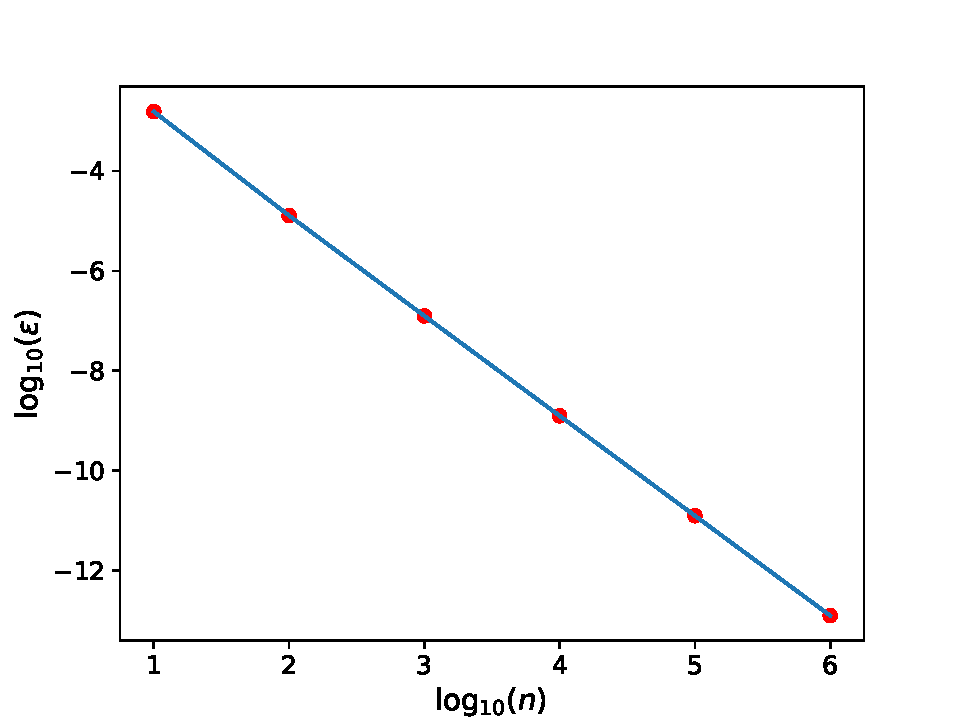
\includegraphics{../imgs/rel_err.pdf}
        \caption{The plot shows the relative error of the numerical approximation $v(x)$ for different numbers of steps.}
        \label{fig:rel_err}
    \end{center}
\end{figure}

\begin{table}%[h!]
    \centering
    \caption{The table shows the maximal relative error in $v(x_i)$, $\max(\epsilon_i)$, for different number of steps, $n_\mathrm{steps}$, used in the numerical approximation.}
    \begin{tabular}{c@{\hspace{1cm}} c}
        \hline
            $n_\mathrm{steps}$ & $\max(\epsilon_i)$ \\
        \hline
            $10$   & $3.3\cdot 10^{-1}$ \\
            $10^2$ & $4.6\cdot 10^{-2}$ \\
            $10^3$ & $6.2\cdot 10^{-3}$ \\
            $10^4$ & $8.5\cdot 10^{-4}$ \\
            $10^5$ & $1.2\cdot 10^{-3}$ \\
            $10^6$ & $6.4\cdot 10^{-3}$ \\
            $10^7$ & $7.4\cdot 10^{-2}$ \\
        \hline
    \end{tabular}\label{tab:max_eps}
\end{table}


\section*{Problem 9}

The algorithm presented in Problem 6 can be specialised for the purpose of the discretised Poisson equation (Eq.~\ref{eq:discPoissonMat}). As we know that $a_i = c_i = -1$ and $b_i = 2$, Algorithm~\ref{algo:triDiagGauss} can be simplified a bit. The result is shown in Algorithm~\ref{algo:PoissonGauss}. The specialised algorithm has
\begin{equation}
    (6n-5) \textrm{ FLOPs}.
    \label{eq:specFlop}
\end{equation}
It is implemented as the function \verb+specAlgo+ in \verb+algo.cpp+. 
\begin{algorithm}[H]
    \caption{Gaussian elimination of Poisson matrix}\label{algo:PoissonGauss}
    \begin{algorithmic}
        \State Initialise $\bv{g}$ with its given values
        \State Initialise new vectors $\bv{v}$ and $\bv{b}$ of length $n$ 

        \Comment Forward substitution
        \State $b_1 = 2$
        \For{$i = 1, 2, \dots, n-1$}                        \Comment $(n-1)$ iterations
            \State $b_{i+1} = 2 - 1/b_i$                    \Comment 2 FLOPs 
            \State $g_{i+1} = g_{i+1} + g_{i}/b_{i}$        \Comment 2 FLOPs 
        \EndFor
        \Comment Backward substitution
        \State $v_n = g_n/b_n$                              \Comment 1 FLOP 
        \For{$i = 1, 2, \dots, n-1$}                        \Comment $(n-1)$ iterations
            \State $v_{n-i} = (g_{n-i} + v_{n-i+1})/b_{n-i}$  \Comment 2 FLOPs
        \EndFor
    \end{algorithmic}
\end{algorithm}


\section*{Problem 10}

Table~\ref{tab:timing} shows the time used for 100 runs of the algorithms. From the number of FLOPs for each of the two algorithms (Eq.~\ref{eq:genFlop} anf \ref{eq:specFlop}) we would expect an relative factor
\begin{equation}
    t_\mathrm{gen}/t_\mathrm{spec} \sim \frac{4}{3}
\end{equation}
between the two algorithms. From our measurements we see that the relative time factor fits quite well with the expectation.

\begin{table}%[h!]
    \centering
    \caption{The table shows the time used, in seconds, for 100 runs of the general and special algorithms, for different numbers of steps. The last coloumn shown the time factor between the two algorithms.}
%    \begin{tabular}{rrrr}
    \begin{tabular}{c@{\hspace{1cm}} c @{\hspace{1cm}} c @{\hspace{1cm}} c}
        \hline
            $n_\mathrm{steps}$ & $t_\mathrm{gen}\, (\mathrm{s})$ & $t_\mathrm{spec}\, (\mathrm{s})$ & $t_\mathrm{gen}/t_\mathrm{spec}$ \\
%            & & & \multicolumn{1}{c}{c} \\
        \hline
            $10$   & $4.62\cdot 10^{-4}$ & $2.54\cdot 10^{-4}$ & $1.82$ \\
            $10^2$ & $2.44\cdot 10^{-3}$ & $1.91\cdot 10^{-3}$ & $1.28$ \\
            $10^3$ & $2.12\cdot 10^{-2}$ & $1.77\cdot 10^{-2}$ & $1.20$ \\
            $10^4$ & $2.27\cdot 10^{-1}$ & $1.20\cdot 10^{-1}$ & $1.15$ \\
            $10^5$ & $1.93$              & $1.57$              & $1.23$ \\
            $10^6$ & $28.7$              & $21.4$              & $1.34$ \\
        \hline
    \end{tabular}\label{tab:timing}
\end{table}


\end{document}
